\chapter{Metodologia}
\label{Cap:MateriaisMetodos}

% Capítulo 3: Materiais e Métodos (ou Metodologia)
\begin{comment}
\indent
\par Este capítulo aborda os materiais e métodos utilizados no projeto, contendo maiores detalhes sobre algoritmos, tecnologias e estratégias empregadas na solução.

\section{Modelo da solução}
\end{comment}

\indent
\par A fim de solucionar o problema identificado, foram definidos métodos e estratégias com o objetivo de criar um fluxo de trabalho. A figura \ref{DiagramaDeBlocosIcones} fornece um diagrama ilustrativo e simplificado da solução proposta.
\begin{comment}
\subsection{Diagramas da solução}

\begin{figure}[H]
    \centering
    \caption{Diagrama de blocos da solução}
    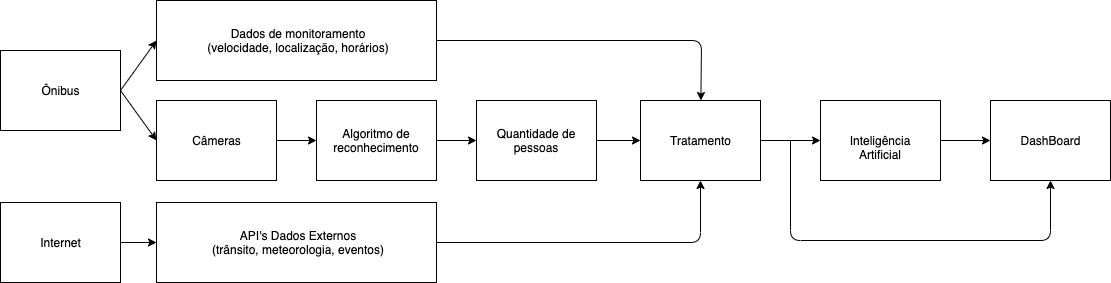
\includegraphics[width=1.0\linewidth]{Imagens/diagramaDeBlocos.jpg}
    \caption*{Fonte: Arquivo dos autores (2020)}
    \label{diagramaDeBlocos}
\end{figure}
\end{comment}

\begin{figure}[H]
    \centering
    \caption{Ilustração da solução}
    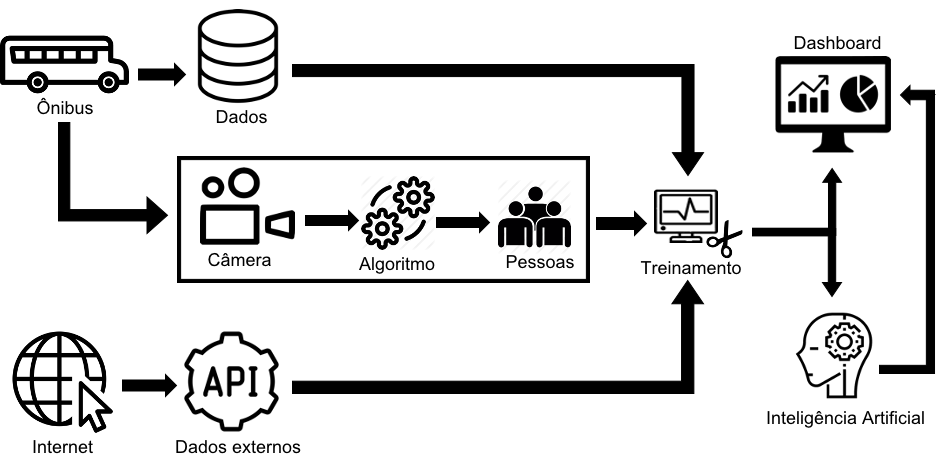
\includegraphics[width=1.0\linewidth]{Imagens/DiagramaDeBlocosIcones.png}
    \caption*{Fonte: Arquivo dos autores (2020)}
    \label{DiagramaDeBlocosIcones}
\end{figure}

\indent
\par Primeiramente alguns dados dos ônibus como por exemplo velocidade, tempo de parada, linhas, posição dos veículos seriam coletados juntamente com imagens do interior dos veículos, que passariam por um algoritmo de reconhecimento para identificar a lotação dos mesmos. Paralelamente, informações obtidas por meio de API's externas enriqueceriam o conjunto de dados, que por sua vez passaria por um tratamento e um treinamento. Após esse processo algumas informações serão direcionadas diretamente para o painel de controle enquanto outras passarão pela inteligencia artificial para depois serem colocadas no dashboard.

\section{Python}
\indent
\par Linguagem de programação de alto nível lançada em 1991. Atualmente possui um modelo de desenvolvimento open source e gerenciado pela Python Software Foundation. A linguagem prioriza a legibilidade de código e possui poderosos recursos advindos de suas bibliotecas padrão combinados com bibliotecas de terceiros.

\section{Pandas}
\indent
\par Biblioteca desenvolvida em Python que possui estruturas de dados que facilitam e agilizam a manipulação e análise de dados.

\section{Numpy}
\indent
\par Biblioteca desenvolvida em Python criada para facilitar o desenvolvimento de aplicações com fins matemáticos e complexidade computacional avançada. Possui suporte para vetores e matrizes multidimensionais e diversas funções matemáticas para interação com essas estruturas.

\section{OpenCV}
\indent
\par Se trata de uma iniciativa open source que teve sua primeira versão lançada nos anos 2000 e continua em expansão até os dias atuais. Atualmente, suporta uma ampla variedade de algoritmos relacionados a Visão Computacional e Machine Learning, além de estar disponível em diversas linguagens de programação como C++, Python, Java e diferentes plataformas como Windows, Linux, OS X, Android e IOS.

\section{Redes Neurais}
\indent
\par Sistemas de computação que tem como objetivo reconhecer e classificar padrões em dados brutos. Tais sistemas buscam agir como o sistema nervoso humano, aprendendo e melhorando continuamente.

\section{YOLO}
\indent
\par Método para detecção e classificação de objetos em uma imagem combinando OpenCV e redes neurais. Se tornou popular pela sua grande eficiência e agilidade quando comparado com outros frameworks desenvolvidos anteriormente.

\section{Django}
\indent
\par Framework de alto nível, gratuito e open source desenvolvido em Python para programação de aplicações web. Apoia o desenvolvimento rápido e limpo, possuindo muitas ferramentas e métodos previamente construídos para facilitar e apoiar o desenvolvedor na criação das aplicações.

\section{Power BI}
\indent
\par Serviço de análise de negócios lançado em 2015 pela Microsoft. Permite a criação e compartilhamento de dashboards para a visualização de dados de forma interativa, além de possuir integração com outras ferramentas, como o Microsoft Excel.


